\documentclass[11pt,a4paper,USenglish,twocolumn]{article}
\usepackage{unir_paper}
\usepackage{subcaption}


%---------------------------
%título del trabajo y autor
%---------------------------
\title{Machine Learning Tools for Open Cluster Characterization with Gaia DR2 Data}
\author{C. D. Álvaro, J. Álvaro, C. A. Guzmán}
\date{24th of January, 2021}


%---------------------------
%marges
%---------------------------
%\usepackage[margin=1.9cm]{geometry}
%---------------------------
%---------------------------
%---------------------------
%---------------------------

\resumen{
The characterization and understanding of \emph{Open Clusters}
allow us to better understand properties and mechanisms about the Universe
such as stellar formation and the kind of regions where these events occur.
They also provide information about stellar processes and the evolution of the galactic disk.

In this paper, we develop a method to characterize open clusters by using
\emph{artificial intelligence} tools, such as clustering by \emph{K-Means}
and clustering based on \emph{Artificial Neural Networks} by implementing
the \emph{Deep Embedded Clustering} model.
We are using \emph{Gaia DR2 database} as data source for testing our models.

The developed method aims to improve current techniques of the state of the art.
We achieve improvements not only in terms of \emph{computational efficiency},
with lower computational requirements, but in \emph{usability},
reducing the number of hyperparameters to obtain a good characterization of the analyzed clusters.

Our method achieves good results,
becoming even better in some cases when the results are compared with current techniques.
}

\palabrasclave{
    characterization,
    data analysis,
    deep embedded clustering,
    gaia,
    machine learning,
    open cluster
}

\begin{document}
\twocolumn[
\begin{@twocolumnfalse}
\maketitle
\end{@twocolumnfalse}
]

%\renewcommand{\listfigurename}{Índice de Ilustraciones}
%\renewcommand{\listtablename}{Índice de Tablas}
%\renewcommand{\contentsname}{Índice de Contenidos}
%\renewcommand{\figurename}{Figura}
%\renewcommand{\tablename}{Tabla}
%\twocolumn


%\frontmatter
%\tableofcontents
%\listoffigures
%\listoftables

\section{INTRODUCTION}

Stellar open clusters (OCs) \cite{janes1982open} are groups of stars
gravitationally bounded originated from a single molecular gas cloud.
They share the same chemical composition and age. Moreover,
they have similar relative positions and proper motion.
Those astronomical objects are relevant to understand the spiral structure,
the dynamics and the chemical evolution of our galaxy.

The study of OCs has been pushed forward thanks to the huge and precise dataset
from the Gaia mission Gaia DR2 available since 2018
\cite{collaboration2016description} and \cite{gaia2018gaia}.
This dataset has helped to review already known open clusters and to find new ones.

Stars that belong to the same OC share relative positions,
inherited from their original gas cloud.
This means that their distances to the Earth are similar for all of them and,
therefore, they have a narrow dispersion in their parallax value.
They also share similar values of proper motion, both in right ascension and declination.
Another property they share is their chemical composition.
Thus, their metallicity must be uniform,
since these stars were born from the same gas cloud and at the same time stage.
However, to take this last property into account, we are faced with the drawback
that this parameter is poorly reported in Gaia DR2 database.

Normally, the characterization process takes into account astrometric features
such as proper motion in right ascension and declination, and parallax.
Photometric features like $E(b-r) / G_{mag}$ are considered too.
These last variables are used for generating the H-R diagram of the OC candidate stars.
This stars should present a sharp profile corresponding to an isochrone curve derived
from a theoretical model.
This model does consider metallicity, mass and brightness of the stars involved.
At the moment, a set of tools have been used for this purpose, as explained later,
but in general, these tools require supervised and parameterized models.
So a previous knowledge of the cluster is necessary or the process must be repeated
iteratively in order to achieve valid results.

Our aim is to build a machine learning model capable of characterizing an open
cluster inside a stellar region with knowing nothing about the region.
This model will take advantage of these features to train an Artificial Neural
Network (ANN) that will clusterize all stars within the given region.
One of these groups will be the open cluster that interests us.
With that purpose we have adapted the Unsupervised Deep Embedding for Clustering
Analysis \cite{xie2016unsupervised} to our problem.

This model fulfills one of our main requirements.
It has to be \emph{non-supervised} and \emph{non-parameterized} in order to make easier
the automation process of analyzing a wide range of regions with different typologies.
Another important requirement for our model is that it must be computationally efficient
in order to run in common workstations.
The model has been developed with Python using the Keras framework which takes
advantage of modern GPUs to make its computations.
That increases significantly the computational capacity of our model making possible
to run it on regular workstations with one of those GPUs.

Since the aim of this work is not to find new OCs but to improve the characterization
of the already known ones, we have taken the approach of analyzing known regions.
These regions have been taken from the OpenClust catalogue \cite{dias2002new}
(see Figure \ref{fig:openclust_catalogue}) and downloaded from Gaia DR2 database
increasing the radius of each region by a factor $1.5$.

\begin{figure}
    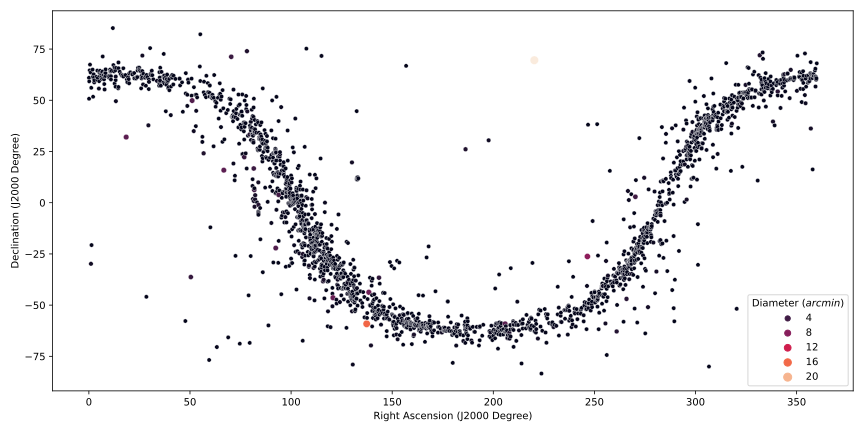
\includegraphics[width=\columnwidth]{../figures/openclust_catalogue.png}
    \caption{OpenClust Catalogue Distribution}
    \label{fig:openclust_catalogue}
\end{figure}

Finally, we have compared the results obtained with the model we purposed with another
method that involves tools from the Virtual Observatory such as Clusterix \cite{balaguer2020clusterix}.

As shown in Section \ref{sec:results}, the results obtained are promising.
This allows us to consider our model as a valid tool that could be part
of the standard set of tools for open clusters characterization.

\section{STATE OF THE ART}

The initial approach to find open clusters is by searching for overdensities
in the astrometric space of the galactic disk and a later identification of
possible OCs using photometric information \cite{castro2020hunting}.
However, although it looks simple, it is not. Here we face the problem that the
near field around the OC is composed of two kind of populations.
The first kind belongs to the membership stars of the OC (from tens or hundreds
to a few thousand) while the second one is composed by a background of stars
that do not belong to the OC (from tens to hundreds of thousands).
To find out which stars do belong to the OC is the problem we try to solve in
this work as this selection is critical to properly characterize the
fundamental properties of the cluster (total mass, age, chemical composition, etc.).

Since the components of the open cluster are born from the same gas cloud and they
share both dynamic properties and relative distance, as well as age and chemical
composition, the first step is to analyze the proper motion configuration space of
the region of interest. This approach is the one used by many tools from the Virtual
Observatory such as TOPCAT \cite{taylor2005topcat}, Clusterix 2.0 \cite{balaguer2020clusterix},
Aladin \cite{bonnarel2000aladin} or VOSA \cite{bayo2008vosa}.

TOPCAT by itself cannot find members of the open cluster. It requires to parameterize
some of the properties of the cluster, what requires a previous knowledge of the cluster.
Or to make a supervised and manual selection of groups based on overdensities
in the proper motion configuration space. Clusterix 2.0, an interactive web-based tool,
can help to this process. It takes the proper motion diagram without making any prior
assumption about the membership of the candidate star and determines empirically
the frequency functions. Clusterix uses normal Gaussian kernel functions, defined as:

\begin{equation*}
  K(a, b) = \frac{1}{2 \pi h^{2}} \exp{ \left[ - \frac{1}{2}\frac{\left( a - a_{i} \right)^{2} + \left( b - b_{i} \right)^{2}}{ h^{2}} \right]}
\end{equation*}

$\left( a, b \right)$ are referred to the proper motion configuration space,
while a point located in the center of the cell $\left( i, j \right)$
provides the maximum contribution for calculating the local density.
Number $h$ is called the \emph{smoothing} parameter and it is measured
in the same units as proper motion.

Clusterix is defined as an unsupervised and non-parameterized tool, but it
critically depends on the selection of three radii.

\begin{itemize}
  \item \textbf{Inner radius} which defines a region with stars that belong to the OC and field stars.
  \item \textbf{Void region}. This region is excluded from the analysis since it is supposed
                to be a transition region with stars that could belong the OC.
  \item \textbf{External region} or field region.
                This is the outer region with stars that do not belong the open cluster.
\end{itemize}

If the analysis performed by Clusterix is successful, it returns the probability
associated to each star in the dataset to belong to the open cluster.
These results can be imported then into TOPCAT to continue the refining process to
get a valid characterization.

Another recent approach to solve this problem based on machine learning techniques
makes a systematic search for overdensities in the astrometric space of the galactic
disk and a subsequent identification of open clusters using photometric information
\cite{castro2020hunting}.

This last method includes two phases: the first one uses an unsupervised clustering
algorithm, DBSCAN, to search for overdensities $(l, b \pi, \mu_{\alpha} *, \mu_{\delta})$,
and then applies a deep learning ANN, previously trained with magnitude diagrams,
to identify isochrone patterns within the detected overdensities and thus proceed
to confirm them as OC.

It should be noted that for the execution of this method, MareNostrum 42
(Barcelona Supercomputing Center) was used.
So the neural network could handle the image recognition process with
isochrone patterns and not applying theoretical models derived from
values such as metallicity or masses, among other.

This work concludes with the identification of 582 new open clusters
distributed along the galactic disk for a galactic declination bellow 20 degrees.
This result increases the number of known open clusters by 45\%.

As told before, our aim in this work, linked to computational limitations compared
to MareNostrum, is not to do a blind search for clusters, but to obtain a method,
in the machine learning environment, that allows the characterization of open clusters.
We require our method to be unsupervised and non-parameterized making it suitable for
automated processes.

We use the Clusterix+TOPCAT method applied to the same clusters that we have analyzed
with our method to validate our results.

In this work we make use of Gaia DR2 since DR3 has not been released in time for us to include it.
Gaia DR2 is a multidimensional dataset obtained by ESA's Gaia mission
(located at L2, 1.5 million kilometers from Earth) and operational since 2014.
The catalogue has high precision and accuracy astrometric data for more than 1.7 billion stellar sources,
and magnitudes in three photometric filters (G, BP and RP) for more than 1,300 million sources.

As we will explain later, what we need to accomplish our aim is an algorithm
that manages to make data groups based on the dynamic properties of the stars.

There are several clustering algorithms: KMeans, Mean-Shift Clustering, DBSCAN \cite{ester1996density}
among other. While each one behaves better according to the distribution of the objects
to clusterize, we have chosen KMeans by its simplicity and good results.

This algorithm works well and gives good results at first approach.
However, we need to set a large number of clusters to find the open cluster we are looking for.
This fact complicates the identification of the OC and many times the found cluster contains to many outliers.
For that reason, we have search for a KMeans refinement based on an artificial neural network.

The \emph{Unsupervised Deep Embedding for Clustering Analysis} model
or \emph{DEC} \cite{xie2016unsupervised} takes KMeans as its starting point,
but then, it trains an autoencoder to reduce the feature space
and pass this transformed data through a Clustering Layer which refines the previous selection.

\section{AIMS AND METHOD}

Our aim is to \emph{build an unsupervised clustering model for open cluster characterization}.
The model will be \emph{non-supervised and non-parameterized} in order to fit a wide range
of clusters without the need for fine-tuning a high number of hyperparameters.

\subsection{DOWNLOAD}

We start by selecting a region from the OpenClust catalogue and downloading it from
Gaia DR2 database into a docker database. This allows us to repeat the analysis without
having to download the data every time. The radius of the downloaded region from Gaia
is 1.5 times larger than the one registered in OpenClust. This way we ensure to include
several stars that do not belong to the open cluster.

\subsection{FEATURE SELECTION}
\label{sec:feature_selection}

As mentioned before, we want our model to characterize open clusters by looking at
their dynamic properties. Also, we want to maintain as simple as possible our
clustering model in order to save computing resources.

Proper motion in right ascension and declination seems like a natural choice since,
as we know, stars belonging to the same OC share a common motion vector.

Parallax is another important feature. It lets us know how far stars are from us.
In addition, since all stars within an open cluster were born from the same dust cloud,
they must all have similar parallax.

However, we are not going to use these raw features.
Instead, we are taking a combination of them.

First, we correct proper motion in right ascension and declination by dividing them by
the parallax. That way, we normalize these quantities and help our clustering models
to improve their performance.

The modulus of the proper motion is another computed property that we are considering.
We use it to relate both features and therefore, to force our model to keep them tight.

\begin{figure}
  \includegraphics[width=\columnwidth]{../figures/melotte_22/features_melotte_22.png}
  \caption{Pairwise relationships among variables using Melotte 22 data}
  \label{fig:features_melotte_22}
\end{figure}

Figure \ref{fig:features_melotte_22} shows a pairwise relationship among some features
available in the dataset for Melotte 22 data.

\subsection{SOFT CLUSTERING}

Our first approach to find the open cluster is using the K-Means algorithm.
Since we are looking for a single cluster, it seems reasonable to use a clustering
algorithm and set it to find two clusters. One for the desired OC and another which
contains stars that do not belong to the open cluster.
However, this idea is not completely right.

\begin{figure}
  \centering
  \begin{subfigure}{\columnwidth}
    \centering
    \begin{subfigure}[t]{0.3\textwidth}
      \centering
      \includegraphics[width=\textwidth]{../figures/kmeans/kmeans_n2_pm_melotte_22.png}
    \end{subfigure}
    \hfill
    \begin{subfigure}[t]{0.3\textwidth}
      \centering
      \includegraphics[width=\textwidth]{../figures/kmeans/kmeans_n5_pm_melotte_22.png}
    \end{subfigure}
    \hfill
    \begin{subfigure}[t]{0.3\textwidth}
      \centering
      \includegraphics[width=\textwidth]{../figures/kmeans/kmeans_n8_pm_melotte_22.png}
    \end{subfigure}
  \end{subfigure}
  \medskip
  \begin{subfigure}{\columnwidth}
    \centering
    \begin{subfigure}[t]{0.3\textwidth}
      \centering
      \includegraphics[width=\textwidth]{../figures/kmeans/kmeans_n2_parallax_melotte_22.png}
      \caption{N = 2}
    \end{subfigure}
    \hfill
    \begin{subfigure}[t]{0.3\textwidth}
      \centering
      \includegraphics[width=\textwidth]{../figures/kmeans/kmeans_n5_parallax_melotte_22.png}
      \caption{N = 5}
    \end{subfigure}
    \hfill
    \begin{subfigure}[t]{0.3\textwidth}
      \centering
      \includegraphics[width=\textwidth]{../figures/kmeans/kmeans_n8_parallax_melotte_22.png}
      \caption{N = 8}
    \end{subfigure}
  \end{subfigure}
  \caption{K-Means comparisons with Melotte 22}
  \label{fig:kmeans_comparisons_melotte_22}
\end{figure}

This is due to the fact that OC's stars are surrounded by other stars with possibly similar
properties. So, setting the number of clusters to two is too low to separate them properly.

As shown in Figure \ref{fig:kmeans_comparisons_melotte_22}, larger values for the number of
clusters allow us to isolate more accurately the resonance in parallax at $\approx 7.3mas$.
However, we have the disadvantage that more groups are formed.

This effect complicates our task of finding the desired open cluster, since we would like
to get just two groups, one for the OC and another with the remaining stars.
Therefore, we have to find a way to set the right value for the number of clusters
to isolate the searched cluster without creating too many groups.

To solve this issue, we will try to estimate the best number of clusters by using the
\emph{silhouette score} \cite{rousseeuw1987silhouettes}.

K-Means does a good job making an initial clustering. However, too many clusters arise
from this characterization and the OC is still polluted with stars that do not belong to it.
Moreover, we would like to reduce the amount of clusters too.

Therefore, we would like to find a better model that improves this initial characterization
by reducing the amount of clusters and also that removes outsiders from the OC.

\subsection{DEC MODEL}

Since we do not have a labeled dataset to train a supervised model,
we have no choice but to use an unsupervised self-trained model.

For that reason we have adapted the \emph{Unsupervised Deep Embedding for Clustering Analysis}
to our work.

The model is composed by a \emph{deep autoencoder}, a \emph{deep encoder} and
a \emph{clustering layer}.

Encoders are used to transform the input data into a latent space
using a non-linear mapping function $f_{\theta} : X \rightarrow Z$.

Although, as explained in section \ref{sec:feature_selection},
the number of features we are managing is not too large,
this latent space helps us reduce the number of features
and avoids the \emph{"curse of dimensionality"} \cite{bellman1961curse}.

These encoders are pretrained before fitting the model to generate predictions. Then,
the encoder is used with the aim of transforming input data to the latent space $Z$. Once the
data has been transformed, a K-Means clusterer is used in order to make an initial clustering.

With that initial configuration, the model iterates alternating between computing an auxiliary
target distribution (Soft Assignment) and minimizing the Kullback-Leiber (KL) divergence
\cite{kullback1951information} to it. This unsupervised algorithm allows us to improve the clustering.

\begin{equation}
  p_{ij} = \frac{q^{2}_{ij} / f_{j}}{\sum_{j'}q^{2}_{ij'}/f_{j'}}
  \label{eq:student_tdistribution}
\end{equation}

In the soft assignment stage,
the \emph{Student's t-distribution} is used as a kernel to measure the similarity
between the embedded points and the cluster centroid.
While in the KL divergence minimization the algorithm iteratively refines clusters by learning
from their high confidence assignments with the help of an auxiliary target distribution.
The model is trained by matching the soft assignment to the target distribution.
The choice of this target distribution is crucial for DEC's performance.
In this work we have taken the target distribution from DEC's original paper \cite{xie2016unsupervised},
which is defined in Equation \ref{eq:student_tdistribution}.

Figure \ref{fig:dec_model_setup} shows the layer setup of our DEC model.
It is simpler than the one tested on the original paper \cite{xie2016unsupervised},
since the number of selected features in our work is smaller than in the original one.
Therefore, using the same configuration would result in a model so
powerful that would incur in overfitting issues unable to make right predictions.

\begin{figure}
  \includegraphics[width=\columnwidth]{../figures/dec_diagram.pdf}
  \caption{DEC model layer setup}
  \label{fig:dec_model_setup}
\end{figure}

Finally, we can refine this selection by filtering those stars which are bellow and above
the 0.10 and 0.90 quantiles for each group, respectively.
That way we remove the most doubtful values from the selection.

All developed resources are available at:
\href{github.com/cdalvaro/machine-learning-master-thesis}{github.com/cdalvaro/machine-learning-master-thesis}

\section{CONTRIBUTION}

\section{RESULTS}
\label{sec:results}

\subsection{Evaluación 1}

\subsection{Evaluación 2 }
En la Tabla \ref{tab_1}
\begin{table}\label{tab_1}
\caption{Unidades de las propiedades magnéticas:}

\begin{tabular}{ccc}\hline\hline
Símbolo & Cantidad & Conversión\\
\hline
$\Phi$ & flujo magnético & $1$Mx $\rightarrow 10^{-8}V\cdot s$\\
... &...&...\\
\hline\hline
\end{tabular}
\end{table}

\section{RESULTS DISCUSSION}

Tras la presentación objetiva de los resultados, querrás aportar una discusión de los mismos.

\section{CONCLUSIONS}

Resumen de las contribuciones del trabajo, en el que relaciones las contribuciones y los resultados obtenidos con los objetivos que habías planteado para el trabajo, discutiendo hasta qué punto has conseguido resolver los objetivos planteados.
Finalmente, hablar de líneas de trabajo futuro que podrían aportar valor añadido al TFM realizado. La sección debería señalar las perspectivas de futuro que abre el trabajo desarrollado para el campo de estudio definido. En el fondo, debes justificar de qué modo puede emplearse la aportación que has desarrollado y en qué campos.

\appendix
\section{APPENDIX}
Apéndices, en caso de ser necesario.

\renewcommand{\refname}{REFERENCES}
\bibliographystyle{unsrt}
\bibliography{references}

\end{document}
